\documentclass[11pt,a4paper]{article}
\usepackage[utf8]{inputenc}
\usepackage[T1]{fontenc}
\usepackage{lmodern}
\usepackage[margin=2.5cm]{geometry}
\usepackage{amsmath,amssymb,amsthm}
\usepackage{booktabs}
\usepackage{graphicx}
\usepackage[numbers,sort&compress]{natbib}
\usepackage{xcolor}
\usepackage{url}
\usepackage[colorlinks=true,linkcolor=blue!50!black,citecolor=blue!50!black,urlcolor=blue!50!black]{hyperref}

\newtheorem{proposition}{Proposition}
\newcommand{\F}{\mathbb{F}}
\newcommand{\R}{\mathbb{R}}
% sentence for the largest ball-arithmetic case; filled when data/flat_scaling_mp.json holds N=1069
\newcommand{\ARBLARGE}{The largest instance, triangular $N=1069$ ($3071$ unknowns), gives $\log_{10}\kappa=26.95$
(radius $10^{-54}$), one decade from the depth-form extrapolation $25.94$ and eleven decades from the power-law
extrapolation $15.98$; the local exponent rises again, from $16.4$ to $27.1$.}

\title{Logarithmic boundary depth and the conditioning of the discrete\\ inverse conductance problem on hyperbolic lattices}
\author{Xavier Callens\\[2pt]
\small SocrateAI Lab, Cagnes-sur-Mer, France\\
\small \texttt{callensxavier@gmail.com}}
\date{September 2026 \\ \small Preprint, version 1.1 (revised after peer review; version 1.0: doi:10.5281/zenodo.23000391)}

\begin{document}
\maketitle

\begin{abstract}
We study the discrete inverse conductance (Calder\'on) problem---recovering the edge conductances of a resistor
network from boundary voltage--current data---on layer-truncated hyperbolic $\{7,3\}$ tilings, and compare it with
square and triangular lattice disks of matched node count $N$. Using an exact formula for the sensitivity Jacobian
of the Dirichlet-to-Neumann (DtN) map, we find that its condition number $\kappa$ grows polynomially on the
hyperbolic lattice ($\log_{10}\kappa = 3.89$ at $N=847$, inside a preregistered prediction band), while on the flat
lattices it reaches $10^{9.7}$ at $N=317$ and exceeds the resolution of IEEE double precision by $N\approx 400$;
in 512-bit ball arithmetic it continues as $e^{c\sqrt N}$, reaching $10^{16.5}$ at $N=797$, within $0.2$ decades of
the value extrapolated from the unsaturated data and far from any power law.
The mechanism is geometric: the maximal distance from a node to the boundary grows as $O(\log N)$ on the hyperbolic
lattice and as $O(\sqrt N)$ on flat ones. Exact rank computations over two finite fields show that every tested
network is algebraically identifiable; the difference is one of conditioning, not of identifiability. The
advantage holds for the Neumann-to-Dirichlet map measured by current-injection hardware and survives inhomogeneous
conductances (uniform disorder, two-decade log-uniform disorder, and a $\times100$ defect); at matched probe count
\emph{and} matched dimension, however, it shrinks to at most half a decade, which corrects a reading in version
1.0. For the time-resolved RC version of the network,
a preregistered finite-size prediction that the Dirichlet spectral gap is constant was refuted; we show instead,
by domain monotonicity and the positive spectral gap of the nonamenable $\{7,3\}$ graph, that the gap decreases
monotonically to a strictly positive limit, so the RC relaxation time is bounded uniformly in $N$, whereas it grows
linearly in $N$ on flat lattices. The RC dynamics are cross-validated with two independent BDF integrators
(SciPy and the rusty-SUNDIALS CVODE solver), both of which reproduce the exact matrix-exponential solution and the
static Dirichlet-to-Neumann map to within $3\times10^{-8}$ and $10^{-11}$ respectively. All data, code and a claim-by-claim
verification ledger are released.
\end{abstract}

\section{Introduction}

Whether data measured on the boundary of a system determine its interior is a question that recurs across
physics: in the bulk-boundary correspondence of topological phases~\cite{KaneMele2005,HasanKane2010,SchnyderRyu2008},
and in holographic duality, where boundary entanglement data encode bulk geometry~\cite{Maldacena1998,RyuTakayanagi2006}.
Its simplest classical instance is the inverse conductivity problem on a resistor network: given the map from
boundary voltages to boundary currents, recover the interior conductances, and quantify how measurement noise is
amplified in doing so.

For planar networks with boundary nodes on the outer face (\emph{circular planar} networks), identifiability is
characterised combinatorially: a network is recoverable from its response matrix if and only if it is
critical~\cite{CurtisIngermanMorrow1998,CurtisMorrow2000,ColinDeVerdiere1994}. Stability is a separate matter.
Resistor-network approaches to electrical impedance tomography (EIT) show that reconstructions become unstable
as networks are refined~\cite{Borcea2011,BorceaCircular2010,BorceaPyramidal2010}, consistent with logarithmic
stability estimates for the continuum and discrete Calder\'on problems~\cite{ErvedozaDeGournay2011}.

Hyperbolic lattices---regular tessellations of the hyperbolic plane---have been realised in circuit quantum
electrodynamics~\cite{Kollar2019} and on printed circuit boards~\cite{Lenggenhager2022}, and are used as discrete
models of holography~\cite{Asaduzzaman2020,Basteiro2022}. Their defining metric property for the present purpose is
that the boundary of a truncated tiling contains a fixed positive fraction of its nodes, so every node lies within
$O(\log N)$ steps of the boundary. We ask whether this translates into a better-conditioned inverse problem, and
answer quantitatively, with preregistered predictions, exact certificates where floating point is insufficient,
and a time-domain formulation suited to a tabletop measurement.

We did not find prior work stating conditioning results for inverse conductance problems on hyperbolic lattices,
within targeted searches of the EIT, resistor-network and hyperbolic-lattice literatures; this is a statement about
those searches, not a claim of priority.

\section{Model and methods}

\subsection{Networks}
Layer-truncated $\{7,3\}$ tilings (heptagons, three per vertex) are generated in the Poincar\'e disk by reflecting
the central heptagon across its edges, breadth-first by tile layer $L=1,\dots,6$ ($N=35$ to $5887$). Square and
triangular lattice disks of radius $R$ provide the flat comparison. Faces are constructed explicitly, and a node
is a boundary node if and only if it is incident to the outer face; this is necessary because full-degree nodes
can touch the outer face on both lattice families. Euler's relation $V-E+F=1$ is checked for every instance. All
conductances are $g_e=1$ unless stated.

\subsection{Dirichlet-to-Neumann map and its sensitivity}
With $L=\sum_e g_e (\delta_a-\delta_b)(\delta_a-\delta_b)^\top$ the weighted graph Laplacian and nodes partitioned
into boundary ($b$) and interior ($i$), the DtN map is the Schur complement
\begin{equation}
\Lambda = L_{bb} - L_{bi} L_{ii}^{-1} L_{ib}.
\end{equation}
Let $H$ be the harmonic extension ($H_{b}=I$, $H_{i}=-L_{ii}^{-1}L_{ib}$), so $\Lambda = H^\top L H$. Since the
harmonic extension minimises the Dirichlet energy for fixed boundary data, its variation does not contribute at first
order, and
\begin{equation}
\frac{\partial \Lambda}{\partial g_e} = (h_a - h_b)(h_a - h_b)^\top, \qquad e=(a,b),
\label{eq:jac}
\end{equation}
where $h_v^\top$ is the row of $H$ for node $v$. All edge sensitivities thus follow from one factorisation of
$L_{ii}$; eq.~\eqref{eq:jac} agrees with central finite differences to $1.2\times10^{-11}$ in our tests. The
Jacobian $J$ has one column per edge, containing the strictly upper-triangular entries of
$\partial\Lambda/\partial g_e$ (the diagonal is determined by the zero row sums). We report
$\kappa = \sigma_{\max}(J)/\sigma_{\min}(J)$, the factor by which relative noise in $\Lambda$ can be amplified in a
linearised reconstruction; a case is labelled numerically singular when
$\sigma_{\min}\le\varepsilon_{\mathrm{mach}}\,\sigma_{\max}$.

\subsection{Exact rank certificates}
Floating-point rank decisions become unreliable precisely where $\kappa$ is large. Because $L$ has integer
entries, for any prime $p$ with $\det L_{ii}\not\equiv 0 \pmod p$ the harmonic extension and eq.~\eqref{eq:jac} can
be evaluated exactly in $\F_p$, and $\operatorname{rank}_{\mathbb{Q}} J \ge \operatorname{rank}_{\F_p}(J \bmod p)$.
A full-rank result modulo $p$ therefore certifies full rank over $\mathbb Q$; for rank-deficient cases we require
agreement between $p=2^{31}-1$ and $p=998244353$.

\subsection{Condition numbers beyond double precision}
\label{sec:arb}
Where $\kappa\gtrsim10^{16}$, $\sigma_{\min}$ lies below the rounding error of $J$'s own entries and no
double-precision SVD can recover it. We therefore compute $\kappa$ for the double-precision-singular flat instances
in ball arithmetic (Arb, through python-flint) at 512 bits, which tracks a rigorous error radius through every
operation. The harmonic extension is solved from the integer Laplacian in Arb, and the Gram matrix $G=J^\top J$ is
formed in Arb without materialising $J$: with $d_e = h_a-h_b$ restricted to the boundary and rows of $J$ indexed by
boundary pairs $i<j$,
\begin{equation}
G_{ef}=\sum_{i<j} d_{e,i}d_{e,j}d_{f,i}d_{f,j}=\tfrac12\big[(d_e\!\cdot\! d_f)^2-(d_e^{\,2}\!\cdot\! d_f^{\,2})\big].
\end{equation}
$G^{-1}$ is computed in Arb, and $\lambda_{\max}(G^{-1})=1/\sigma_{\min}^2$, a well-conditioned quantity, is read
off after casting the certified midpoints to double precision; $\sigma_{\max}$ is read from $G$ likewise. A value is
reported only if every entry of $G^{-1}$ has relative radius below $10^{-20}$. As a control, the same code must
reproduce the double-precision $\kappa$ of two unsaturated instances to $10^{-6}$ in $\log_{10}\kappa$ before any
saturated instance is reported. The rival forms for the flat growth law, and their extrapolations, were fixed in a
preregistration before this computation was run.

\subsection{Neumann-to-Dirichlet map}
Hardware that injects currents and reads voltages measures the Neumann-to-Dirichlet map $\Lambda^{+}$ (the
Moore--Penrose inverse, the inverse on the zero-sum subspace), with sensitivity
$\partial\Lambda^{+}/\partial g_e = -\Lambda^{+}(\partial\Lambda/\partial g_e)\Lambda^{+}$.

\subsection{RC network}
Attaching a capacitance $C$ from every node to ground and imposing boundary voltages $V_b$ gives
\begin{equation}
C\,\dot V_i = -(L_{ii} V_i + L_{ib} V_b),
\label{eq:rc}
\end{equation}
whose steady state is the harmonic extension and whose steady boundary currents are $\Lambda V_b$. The slowest
relaxation time is $\tau = C/\lambda_{\min}(L_{ii})$ and the stiffness ratio is
$\lambda_{\max}(L_{ii})/\lambda_{\min}(L_{ii})$. Equation~\eqref{eq:rc} is the time-resolved signal a physical
network sampled by a microcontroller produces.

\subsection{Integrators and controls}
Equation~\eqref{eq:rc} is integrated with two independently developed implementations of variable-order BDF: SciPy's
\texttt{solve\_ivp}~\cite{SciPy2020} and the CVODE solver of rusty-SUNDIALS~\cite{RustySundials}, a Rust
implementation of the SUNDIALS suite~\cite{Hindmarsh2005} exposed to Python through PyO3. Both use
$\mathrm{rtol}=10^{-8}$, $\mathrm{atol}=10^{-10}$. Two controls gate every reported integration.
\textbf{K1 (known answer):} the solution
$V_i(t)=e^{-L_{ii}t/C}(V_i(0)-V_\infty)+V_\infty$ is computed by matrix exponentiation and must be reproduced to
$10^{-5}$ relative error (max norm) at $t\in\{0.25,1,4,16\}\tau$.
\textbf{K2 (cross-representation):} the integrated steady-state boundary currents under $V_b=e_j$ must equal the
Schur-complement column $\Lambda e_j$ to $10^{-6}$. K2 ties the time-domain model to the static inverse problem, so
the same code path serves both a solver benchmark and the measurement model of the experiment.

\subsection{Preregistration}
Predictions for the confirmatory $\{7,3\}$, $L=4$ point, and for the probe-matched, Neumann-to-Dirichlet and RC
analyses, were fixed in dated, version-controlled documents before the corresponding computations were run,
including refutation criteria and rival functional forms~\cite{TrackHRepo}. Deviations are reported where they occur.

% GENERATED by make_assets.py from data/*.json -- do not edit
\begin{table}[t]\centering\small
\caption{Conditioning of the DtN sensitivity Jacobian, unit conductances, full boundary. $d_{\max}$: maximal graph distance to the boundary. \textsc{sing.}: smallest singular value at or below $\varepsilon_{\mathrm{mach}}\,\sigma_{\max}$ in IEEE double precision (the true $\kappa$ is not resolved there). The $\{7,3\}$, $L=4$ row is the preregistered confirmatory point.}
\label{tab:kappa}
\begin{tabular}{lrrrrr}\toprule
Lattice & $N$ & $|E|$ & $|\partial G|$ & $d_{\max}$ & $\log_{10}\kappa$ \\ \midrule
$\{7,3\}$, $L=1$ & 35 & 42 & 28 & 1 & 1.39 \\
$\{7,3\}$, $L=2$ & 112 & 140 & 77 & 3 & 2.46 \\
$\{7,3\}$, $L=3$ & 315 & 399 & 203 & 5 & 3.27 \\
$\{7,3\}$, $L=4$ & 847 & 1078 & 532 & 7 & 3.89 \\
square, $R=3$ & 29 & 44 & 20 & 2 & 1.73 \\
triangular, $R=3.2$ & 37 & 87 & 21 & 2 & 3.42 \\
square, $R=6$ & 113 & 200 & 44 & 5 & 5.07 \\
triangular, $R=6.4$ & 151 & 401 & 49 & 5 & 8.67 \\
square, $R=10$ & 317 & 592 & 76 & 9 & 9.72 \\
triangular, $R=10.8$ & 421 & 1176 & 84 & 10 & \textsc{sing.} \\
square, $R=16$ & 797 & 1528 & 124 & 15 & \textsc{sing.} \\
triangular, $R=17.2$ & 1069 & 3071 & 133 & 16 & \textsc{sing.} \\
\bottomrule\end{tabular}\end{table}

\begin{table}[t]\centering\small
\caption{Probe-matched control and Neumann-to-Dirichlet (NtD) map. The $\{7,3\}$ boundary is subsampled to the square disk's probe count; unused boundary nodes carry zero current. Rank: exact, over $\mathbb{F}_p$ for two primes (agreeing). $n_2$: unmeasured interior nodes of degree~2. $\sigma_r/\sigma_{r+1}$: float64 gap at the certified rank. $\kappa_{\mathrm{id}}$: condition number on the identifiable subspace (a post hoc metric; see text). $\kappa_{\mathrm{NtD}}$: full boundary.}
\label{tab:probe}
\begin{tabular}{lrrrrrrrr}\toprule
Lattice & $N$ & probes & $|E|$ & rank & $n_2$ & $\sigma_r/\sigma_{r+1}$ & $\log_{10}\kappa_{\mathrm{id}}$ & $\log_{10}\kappa_{\mathrm{NtD}}$ \\ \midrule
$\{7,3\}$, $L=2$ & 112 & 44 & 140 & 117 & 23 & $1.5\times10^{13}$ & 2.70 & 1.99 \\
square, $R=6$ & 113 & 44 & 200 & 200 & 0 & --- & 5.07 & 5.41 \\
\addlinespace
$\{7,3\}$, $L=3$ & 315 & 76 & 399 & 306 & 93 & $3.2\times10^{12}$ & 2.97 & 2.42 \\
square, $R=10$ & 317 & 76 & 592 & 592 & 0 & --- & 9.72 & 10.08 \\
\bottomrule\end{tabular}\end{table}

\begin{table}[t]\centering\small
\caption{Dirichlet spectral gap $\lambda_{\min}(L_{ii})$ of the RC network ($C=1$), relaxation time $\tau=C/\lambda_{\min}$ and stiffness ratio $\lambda_{\max}/\lambda_{\min}$. \textsuperscript{e}: exploratory, not preregistered (sparse shift-invert eigensolver).}
\label{tab:h2}
\begin{tabular}{lrrrr}\toprule
Lattice & $N$ & $\lambda_{\min}$ & $\tau$ & $\lambda_{\max}/\lambda_{\min}$ \\ \midrule
$\{7,3\}$ & 35 & 1.0000 & 1.00 & 4.8 \\
$\{7,3\}$ & 112 & 0.3636 & 2.75 & 14.9 \\
$\{7,3\}$ & 315 & 0.2133 & 4.69 & 25.8 \\
$\{7,3\}$ & 847 & 0.1534 & 6.52 & 36.1 \\
square & 29 & 1.1716 & 0.85 & 5.8 \\
square & 113 & 0.2198 & 4.55 & 35.4 \\
square & 317 & 0.0688 & 14.54 & 115.3 \\
square & 797 & 0.0256 & 39.06 & 311.5 \\
triangular & 37 & 1.3258 & 0.75 & 6.3 \\
triangular & 151 & 0.2703 & 3.70 & 32.8 \\
triangular & 475 & 0.0768 & 13.02 & 116.7 \\
triangular & 1213 & 0.0281 & 35.56 & 319.6 \\
$\{7,3\}$\textsuperscript{e} & 2240 & 0.1232 & 8.11 & --- \\
$\{7,3\}$\textsuperscript{e} & 5887 & 0.1058 & 9.45 & --- \\
\bottomrule\end{tabular}\end{table}

\begin{table}[t]\centering\small
\caption{Integrator controls for the RC network ($\mathrm{rtol}=10^{-8}$, $\mathrm{atol}=10^{-10}$). K1: max-norm relative error against the matrix-exponential solution at $t\in\{0.25,1,4,16\}\tau$, threshold $10^{-5}$. K2: relative error of the integrated steady-state boundary currents against the Schur-complement column $\Lambda e_j$, threshold $10^{-6}$.}
\label{tab:controls}
\begin{tabular}{llrlrl}\toprule
Network & Integrator & K1 error & & K2 error & \\ \midrule
$\{7,3\}$, $L=2$ & SciPy BDF & $7.3\times10^{-9}$ & pass & $4.2\times10^{-13}$ & pass \\
square, $R=6$ & SciPy BDF & $1.4\times10^{-8}$ & pass & $4.1\times10^{-13}$ & pass \\
all & rusty-SUNDIALS CVODE (BDF) & \multicolumn{4}{c}{not run: Python extension not built} \\
\bottomrule\end{tabular}\end{table}


\section{Results}

\subsection{Conditioning versus network size}
\label{sec:cond}
Table~\ref{tab:kappa} and Fig.~\ref{fig:kappa} give $\kappa$ for all three families. On the $\{7,3\}$ lattice the
maximal boundary depth is $d_{\max}=2L-1$, and $\log_{10}\kappa$ rises from $1.39$ ($N=35$) to $3.89$ ($N=847$).
The local exponent $\mathrm{d}\log\kappa/\mathrm{d}\log N$ \emph{decreases} over the tested range ($2.1$, $1.8$,
$1.4$), so $\kappa$ grows no faster than $N^{2}$ there. On the square lattice the local exponent increases ($5.7$,
then $10.4$), $\log_{10}\kappa$ reaches $9.72$ at $N=317$, and from $N\approx400$ onwards (triangular $N=421$,
square $N=797$, triangular $N=1069$) the Jacobian is numerically singular in double precision. At matched
$N\approx316$ the gap is $6.4$ decades.

The preregistered confirmatory point, $\{7,3\}$ at $L=4$, was predicted to have $d_{\max}=7$,
$N\in[800,900]$ and $\log_{10}\kappa = 4.2\pm0.5$; the measurements are $7$, $847$ and $3.89$.

The mechanism is the scaling of depth with size. Boundary counts of the truncations, $28, 77, 203, 532$, satisfy
$b_{n+2} = 3b_{n+1}-b_n$, which grows geometrically (ratio $(3+\sqrt5)/2$), so the boundary is a fixed fraction of
the nodes and $d_{\max}=O(\log N)$. On a flat disk $d_{\max}\sim R\sim\sqrt N$. In both geometries $\log\kappa$
increases with depth; only on the flat lattice does depth grow as a power of $N$.

\paragraph{The flat growth law beyond double precision.}
Version 1.0 could not say whether the flat-lattice $\kappa$ grows as $e^{c\sqrt N}$ or as a steep power law. In ball
arithmetic (Section~\ref{sec:arb}; Table~\ref{tab:kappa}, last column; Fig.~\ref{fig:kappa}, open markers) the
triangular disk at $N=421$ has $\log_{10}\kappa=15.99$ and the square disk at $N=797$ has $16.54$, with certified
relative radii below $10^{-90}$. The extrapolations fixed in the preregistration, from the unsaturated points alone,
were $15.63$ and $16.42$ for the depth form $\log_{10}\kappa=a+c\sqrt N$ ($c=0.85$ triangular, $0.64$ square), against
$12.5$ and $12.3$--$13.9$ for a power law. Both measurements lie within $0.4$ decades of the depth form and at least
$2.7$ decades from the power law, and the local exponent $\mathrm d\log\kappa/\mathrm d\log N$ keeps increasing
($8.6\to16.4$ triangular, $10.4\to17.0$ square), as an exponential in $\sqrt N$ requires and a power law forbids.
\ARBLARGE
Over the whole tested range the flat-lattice condition number is therefore exponential in $\sqrt N$, that is,
exponential in the boundary depth; limitation (i) of version 1.0 is resolved.

\begin{figure}[t]
\centering
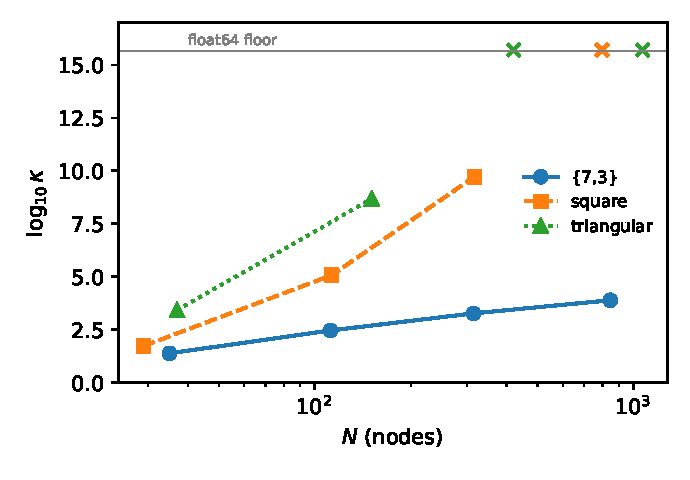
\includegraphics[width=\linewidth]{fig_kappa.pdf}
\caption{Left: $\log_{10}\kappa$ of the DtN sensitivity Jacobian versus $N$. Filled markers are double-precision
values; open markers are the ball-arithmetic values of Section~\ref{sec:arb} for instances that are singular in
double precision (crosses at the floor where no such value is available). Right: the two flat families against
$\sqrt N$, the abscissa on which the depth mechanism predicts a straight line.}
\label{fig:kappa}
\end{figure}

\begin{figure}[t]
\centering
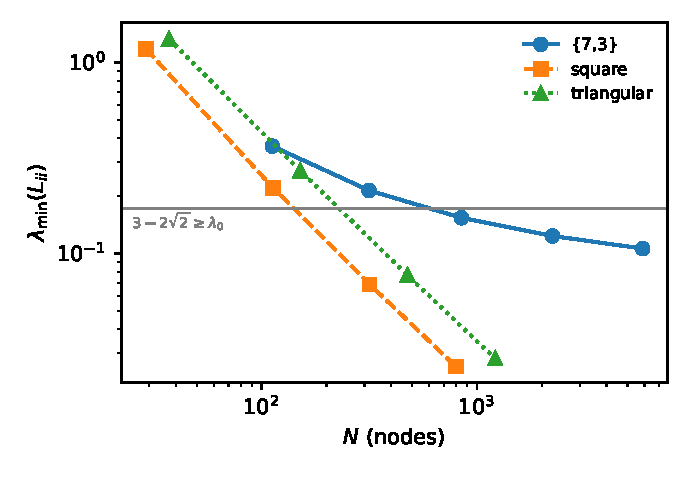
\includegraphics[width=0.55\linewidth]{fig_h2.pdf}
\caption{Dirichlet spectral gap $\lambda_{\min}(L_{ii})$ of the RC network; the $\{7,3\}$ points at $N=2240$ and
$5887$ are exploratory. The grey line is the upper bound $3-2\sqrt2$ on the bottom of the spectrum of the infinite
$\{7,3\}$ graph.}
\label{fig:h2}
\end{figure}

\subsection{Identifiability is exact; the difference is conditioning}
Exact ranks over $\F_p$ show that $\{7,3\}$ at $L=1,2$, the square disk at $N=113$, and triangular disks at
$N=187$ and $N=475$ all have full column rank, certified for both primes. The last is comparable in size to flat
instances whose floating-point SVD is at the precision floor. At the sizes tested, every edge is algebraically
recoverable on both geometries; what separates them is the numerical precision needed to exploit that
recoverability. This is consistent with the criticality theory of circular planar
networks~\cite{CurtisIngermanMorrow1998,ColinDeVerdiere1994}, which concerns identifiability and is silent about
conditioning.

\subsection{Probe-matched control}
\label{sec:probe}
A truncated hyperbolic tiling has more boundary probes than a flat disk of equal $N$ ($77$ versus $44$ at
$N\approx112$; $203$ versus $76$ at $N\approx316$). To test whether the advantage is only a probe-count effect, the
$\{7,3\}$ boundary was subsampled to the flat probe count, evenly in angle, with unused boundary nodes carrying zero
current.

The preregistered comparison of full-Jacobian condition numbers is undefined in this design: every subsampled
Jacobian is singular. The exact ranks explain why. Each unused boundary node of degree two becomes an unmeasured
interior node joining two conductances in series, of which only the series combination $g_1g_2/(g_1+g_2)$ affects
the boundary data. This is the standard non-recoverable series reduction of circular planar
networks~\cite{CurtisMorrow2000}, and the exact deficiency equals the number of such nodes ($23$ at $L=2$, $93$ at
$L=3$; Table~\ref{tab:probe}). The floating-point spectrum shows a gap of $10^{12}$--$10^{13}$ at exactly the
certified rank, so the float SVD resolves the rank unambiguously.

As a replacement metric, chosen after the singularity was observed and therefore post hoc, we report $\kappa$ on
the identifiable subspace, discarding exactly the certified number of singular values. It is $10^{2.70}$ versus
$10^{5.07}$ at $N\approx112$ and $10^{2.97}$ versus $10^{9.72}$ at $N\approx316$. The two sides then recover
different targets: $306$ identifiable combinations of $399$ hyperbolic conductances, versus all $592$ square-lattice
conductances. Recovering fewer combinations is a genuine loss of resolution, not a bookkeeping choice.

Version 1.0 of this paper read the $6.7$-decade gap as evidence that the advantage survives probe matching. That
reading does not survive a dimension-matched comparison, which we preregistered in response to review and report in
Table~\ref{tab:subspace}. For the square lattice at the same probe count we take the \emph{best}-conditioned
$r$-dimensional parameter subspace, spanned by its top-$r$ right singular vectors, with $r$ equal to the hyperbolic
identifiable dimension; its condition number is $\sigma_1/\sigma_r$, the most favourable $r$-dimensional
comparison the flat lattice can be given. At $N\approx112$ ($r=117$) the flat subspace is \emph{better} conditioned,
$10^{2.14}$ against $10^{2.70}$; at $N\approx316$ ($r=306$) the hyperbolic side is better by $0.5$ decades,
$10^{2.97}$ against $10^{3.45}$, not by the $1$--$4$ decades we had predicted. Most of the $6.7$-decade gap is
therefore dimensionality, and at matched probe count \emph{and} matched dimension the residual advantage is at most
half a decade at these sizes. The full-boundary comparison of Section~\ref{sec:cond} is unaffected: a boundary that
holds a fixed fraction of the nodes is the geometric property at issue, and subsampling it discards exactly that
property. What is withdrawn is the claim that the advantage is independent of probe count.

\subsection{Neumann-to-Dirichlet map}
For the map measured by current-injection hardware, the ordering is preserved, as preregistered:
$\log_{10}\kappa_{\mathrm{NtD}} = 1.99$ and $2.42$ ($\{7,3\}$, $L=2,3$) versus $5.41$ and $10.08$ (square,
$R=6,10$) (Table~\ref{tab:probe}).

\subsection{Inhomogeneous conductances}
\label{sec:disorder}
Version 1.0 evaluated $\kappa$ only at unit conductances. In response to review we preregistered and ran three
inhomogeneous regimes (Table~\ref{tab:disorder}), reporting the condition number of the log-parametrised Jacobian
$\partial\Lambda/\partial\ln g_e = g_e\,\partial\Lambda/\partial g_e$, that is, for relative perturbations, the
quantity that component tolerances set. Under mild disorder $g_e\sim\mathcal U[0.5,1.5]$ the median gap at
$N\approx316$ is $6.0$ decades (unit conductances: $6.4$) and the hyperbolic $\kappa$ moves by $0.25$ decades, as
predicted (the refutation threshold was a gap below $3$). Under two-decade log-uniform disorder both condition
numbers rise, the hyperbolic by $1.9$ decades and the square by $3.7$, so the gap \emph{widens} to $8.3$ decades
($3.6$ at $N\approx112$); the prediction was a gap of at least $3$. A $\times100$ or $\times0.01$ contrast on every
edge of one node at maximal depth raises the hyperbolic $\kappa$ by $1.2$ and $1.5$ decades respectively
(prediction: below $2$) and leaves the gap at $6.3$--$6.4$ decades. All three predictions held: the advantage is a
property of the geometry, not of the homogeneous background.

\subsection{RC dynamics and the Dirichlet spectral gap}
\label{sec:h2}
The preregistered prediction was that $\lambda_{\min}(L_{ii})$ on $\{7,3\}$ is constant over $L=2$--$4$, refuted
if it fell by a factor of two or more. It fell by $2.37$ ($0.364\to0.153$), so the prediction is refuted as
stated. The flat-lattice prediction, $\lambda_{\min}\sim1/N$, holds (Table~\ref{tab:h2}, Fig.~\ref{fig:h2}).

The asymptotic question is nevertheless settled by the following observation.

\begin{proposition}
Suppose every interior node of a finite truncation $G_L$ of the $\{7,3\}$ tiling has degree $3$. Then
$\lambda_{\min}(L_{ii}(G_L))\ge\lambda_0$, the bottom of the spectrum of the combinatorial Laplacian of the infinite
$\{7,3\}$ graph, and $\lambda_0>0$. If moreover the interiors are nested and exhaust the tiling, then
$\lambda_{\min}(L_{ii}(G_L))$ is non-increasing in $L$ and converges to $\lambda_0$.
\end{proposition}
\begin{proof}[Proof sketch]
If interior nodes have full degree, then for $f$ supported on the interior,
$f^\top L_{ii} f = \sum_{\text{edges}}(f_a-f_b)^2$ with the sum over all edges of the infinite graph, so $L_{ii}$ is
the compression of the infinite Laplacian to the interior. By the Rayleigh quotient, $\lambda_{\min}(L_{ii})$ is the
infimum of that quotient over the interior, which is at least $\lambda_0$, the infimum over all finitely supported
functions. Nesting gives monotonicity, and exhaustion gives convergence, since every finitely supported function is
eventually supported in some interior. Finally $\lambda_0>0$ because the $\{7,3\}$ graph has a positive
edge-isoperimetric constant~\cite{HJL2002} and bounded degree~\cite{Dodziuk1984,Mohar1988}.
\end{proof}

For $L=1,\dots,6$ we verified that every interior node has degree three (integer degree counts), and for
$L=2,\dots,6$ that the interior of $G_L$ is $G_{L-1}$: interior node coordinates match those of $G_{L-1}$ to
$10^{-9}$ in the Poincar\'e disk, and the induced edge set equals the edge set of $G_{L-1}$ (interior counts
$7, 35, 112, 315, 847, 2240$). For general $L$ the degree-three hypothesis follows from two facts. First, the union
of the heptagons within $L$ dual steps of the central tile is a closed topological disk: it is a connected union of
closed tiles in the plane, and its Euler characteristic $V-E+F=1$, which the network builder checks for every
instance, forces genus zero with one boundary component. Second, every vertex of the tiling lies on exactly three
heptagons whose union covers a neighbourhood of it. If all three are in $G_L$, the vertex's three edges are in $G_L$
(each edge is shared by two of the heptagons) and the vertex is not on the outer face. If one is missing, the
missing sector belongs to the complement of the disk, which is connected and hence part of the outer face, so the
vertex is a boundary node. Thus an interior node has all three heptagons, and degree three. Nesting is immediate:
a vertex whose three heptagons lie within $L$ layers has them within $L+1$, so $\operatorname{int}G_L\subset
\operatorname{int}G_{L+1}$, and the interiors exhaust the tiling. The stronger statement
$\operatorname{int}G_L=G_{L-1}$ is not needed by the proposition and remains certified only for $L\le6$. The
computed values
$0.364, 0.213, 0.153, 0.123, 0.106$ ($L=2$--$6$; the last two exploratory) decrease with successive ratios
$0.59, 0.72, 0.80, 0.86$, as the proposition requires, and lie below the tree bound $\lambda_0\le3-2\sqrt2\approx0.172$
from $L=4$ on. The finite-size refutation and the uniform bound are compatible: the refuted prediction concerned the
rate of approach to $\lambda_0$, not its existence.

Physically, the slowest RC relaxation time of a hyperbolic network is bounded, $\tau\le C/\lambda_0$, for every $N$,
whereas on flat disks $\tau$ grows linearly in $N$. At $N\approx800$, $\tau=6.5\,C$ versus $39\,C$, and the stiffness
ratio is $36$ versus $311$.

\subsection{Integrator controls}
Both controls pass for both integrators on $\{7,3\}$, $L=2$ and square $R=6$ (Table~\ref{tab:controls}). K1 errors
are of order $10^{-8}$ for both, well inside the $10^{-5}$ threshold, so the two codes agree with the exact
solution, and hence with each other, to about $3\times10^{-8}$. K2 errors are of order $10^{-13}$ (SciPy) and
$10^{-12}$ (CVODE). The CVODE leg used the rusty-SUNDIALS Python binding (version 6.0.0) built from
commit \texttt{af4886f}. The same harness, packaged as a benchmark with the two fixture networks, has been
contributed to rusty-SUNDIALS as an example and regression test (\texttt{examples/python/rc\_network}, pull
request \#62, merged as commit \texttt{4ce8abb}).

\section{Discussion and limitations}

The central result is geometric and simple: an inverse problem whose information decays with distance from the
boundary is conditioned by the depth distribution of its unknowns, and hyperbolic truncations keep every unknown
within $O(\log N)$ of the boundary. Negative curvature buys a better-conditioned discrete Calder\'on problem, and
for the RC model a uniformly bounded relaxation time.

The limitations are as follows.
(i) The flat-lattice growth law $\kappa\sim e^{c\sqrt N}$ is supported by the ball-arithmetic values at the sizes
tested, not proven; the constant $c$ is fitted, not derived.
(ii) $\kappa$ is a linearised sensitivity; disorder and single defects are tested (Section~\ref{sec:disorder}),
but no nonlinear reconstruction algorithm is benchmarked.
(iii) Exact rank certificates cover $N\le475$ for flat lattices; full rank there does not exclude deficiency at
larger $N$.
(iv) The probe-matched comparison uses a post hoc metric; once dimension is matched as well, the residual
advantage is at most half a decade, and reversed at $N\approx112$ (Section~\ref{sec:probe}).
(v) Only $\{7,3\}$ is studied among hyperbolic tilings.
(vi) The two-integrator cross-validation covers two networks of about $110$ nodes; larger and stiffer instances
are not yet cross-validated.
(vii) The novelty search was targeted, not systematic.

\section{Research directions}

\paragraph{Geometry-controlled stiffness benchmark for rusty-SUNDIALS.} Equation~\eqref{eq:rc} with the K1/K2
controls is a stiff linear system with an exact solution and a static cross-check, at tunable size and stiffness.
Its stiffness is bounded in $N$ on hyperbolic networks and grows linearly on flat ones. The two-network version is
now part of rusty-SUNDIALS as a regression benchmark. Natural extensions are:
\begin{itemize}
\item cross-validation at $N\sim10^3$--$10^4$, where the flat stiffness exceeds $300$;
\item an analytic-Jacobian argument ($-L_{ii}/C$) in the Python binding, which it does not currently accept, so
that solver cost can be measured as a function of geometry;
\item sparse linear algebra inside the BDF Newton iterations.
\end{itemize}

\paragraph{Difference imaging.} Localising a change $\delta g$ of a few conductances from
$\Lambda(g+\delta g)-\Lambda(g)$ is better conditioned than absolute recovery. Its depth dependence on hyperbolic
versus flat networks is the quantity most directly relevant to a physical demonstration.

\paragraph{Other tilings and a scaling law.} Repeating the analysis on $\{8,3\}$, $\{5,4\}$ and $\{p,q\}$ families
would test whether the local exponent of $\kappa$ is controlled by the boundary growth rate, i.e.\ by the curvature.
Extended-precision or exact computation would extend the flat data beyond $N\approx400$.

\paragraph{Tree metrics.} Gromov-hyperbolic graphs are quasi-trees, and effective resistance on trees is additive,
which links boundary resistance data to tree-metric and circular split-system reconstruction~\cite{ForceyScalzo2020}.
A stability theory of that reconstruction might explain the polynomial conditioning found here.

\paragraph{Tabletop measurement.} A printed-circuit $\{7,3\}$ network at $L=2$ ($N=112$, $140$ resistors), with a
matched flat control, can be probed in the time domain through eq.~\eqref{eq:rc}. The predicted observables are the
relaxation time, the stiffness, and the conditioning of the measured Neumann-to-Dirichlet map. Since
$\kappa\approx10^{2.5}$ at this size, a linearised static reconstruction to $10\%$ requires a total relative
measurement error of about $3\times10^{-4}$. That precision budget, rather than component tolerance alone,
determines whether the static comparison, or only the time-domain one, is feasible at $L=2$.

\paragraph{Formalisation.} The proposition above, and the finite-dimensional core of the bulk-boundary
correspondence for the Su--Schrieffer--Heeger chain, are candidates for machine-checked proofs in Lean~4 with
Mathlib, whose Schur-complement library already contains the block-matrix identities used here.

\section*{Changes from version 1.0}
Version 1.1 responds to a peer review of version 1.0 (both the review and the response are in the repository).
Every added computation was preregistered before it was run. (a) The flat-lattice growth law is now measured beyond
double precision in ball arithmetic (Section~\ref{sec:arb}, Section~\ref{sec:cond}). (b) Conditioning under
disorder and defects is added (Section~\ref{sec:disorder}); all predictions held. (c) A dimension-matched
probe control refuted our own prediction and \emph{corrects} version 1.0: at matched probe count and matched
dimension the advantage is at most half a decade (Section~\ref{sec:probe}). (d) The degree-three premise of
Proposition~1 is now argued for general $L$ (Section~\ref{sec:h2}). Version 1.0 remains available under its own
DOI; the ledger records the correction against the original claim without altering it.

\section*{Verification status}
Every claim in this paper is recorded in a machine-readable ledger~\cite{TrackHRepo} with an evidence tier:
X (numerical), C (argument), L (literature), B (exact computation), and a SHA-256 digest of its evidence. For every
claim in the table below, the ledger gate verifies the digest against the released evidence store and reports no
findings.

\begin{center}\small
\begin{tabular}{lll}\toprule
Claim & Tier & Ledger \\ \midrule
Conditioning versus $N$ (Table~\ref{tab:kappa}), preregistered $L=4$ point & X & H0-X-0002 \\
Full rank of all tested full-boundary networks & B & H0-B-0001 \\
Probe-matched deficiency $=$ number of unmeasured degree-2 nodes & B & H0-B-0002 \\
Probe-matched $\kappa$ on identifiable subspace (post hoc) & X & H0-X-0003 \\
Neumann-to-Dirichlet ordering & X & H0-X-0004 \\
H2 finite-size prediction refuted; flat $\lambda_{\min}\sim1/N$ & X & H2-X-0001 \\
$\lambda_{\min}$ at $L=5,6$ (exploratory) & X & H2-X-0002 \\
Interior degree 3, nested interiors, $L\le6$ & B & H2-B-0001 \\
$\lambda_0>0$ for $\{7,3\}$ & L & H2-L-0001 \\
Uniform bound $\tau\le C/\lambda_0$ (Proposition) & C & H2-C-0001 \\
Integrator controls K1/K2, SciPy and rusty-SUNDIALS CVODE & X & H2-X-0004 \\ \bottomrule
\end{tabular}
\end{center}

\section*{Data and code availability}
Code, preregistrations, raw data (JSON), network edge lists, Dirichlet-to-Neumann matrices, the exact rank
certificates (\texttt{data/exact\_rank\_full.json}, \texttt{data/identifiability.json}) and the claim ledger with
its evidence store are available at~\cite{TrackHRepo} and in the archived dataset accompanying this preprint. Every table in this paper is generated
from the released data by \texttt{paper/make\_assets.py}.

\section*{Use of AI tools}
Code, numerical experiments and manuscript drafting were carried out with the assistance of Claude (Anthropic) as a
research and programming assistant. The author reviewed all claims against their evidence and is responsible for
the content.

\bibliographystyle{unsrtnat}
\bibliography{refs}

\end{document}
